\documentclass{beamer}
\usepackage[czech]{babel}
\usepackage[utf8x]{inputenc}
\usetheme{Malmoe}


\title{Typografie a~publikování}
\subtitle{SAPO\,--\,Samočinný počítač}
\author{Tomáš Coufal}
\institute{Fakulta informačních technologií \\ Vysoké učení technické v~Brně}
\date{\today}

\begin{document}
\section{Úvod}
\frame{\titlepage}
\subsection{Obsah}
    \begin{frame}
        \frametitle{Obsah}
        \tableofcontents
    \end{frame}
\subsection{Úvod}
    \begin{frame}
      \frametitle{Úvod}
      \begin{itemize}
          \item Pro tuhle krátkou prezentaci jsem zvolil téma z české historie informatiky
          \item Období působení pana prof. Svobody na ČVUT je jedno z nejzajímavějších, co může naše historie nabídnout
          \item Díky jeho práci jsem v mnohém předčili celý svět, ale kvůli politické situaci to bylo pohřbeno
      \end{itemize}
    \end{frame}
\section{SAPO\,--\,po stránce historické}
\subsection{Historické souvislosti}
    \begin{frame}
        \frametitle{Historické souvislosti}
        \begin{itemize}
            \item Doba 50.\,let 20.\,století, politické situace v ČSSR nebyla vědecké práci moc nakloňena
                \begin{itemize}
                    \item Zvláště pro lidi jako prof. Svoboda, kteří za války působili na Západě
                \end{itemize}
            \item Kybernetika byla výslovně zakázána samotným Stalinem
            \item Neexistujicí pracoviště, nový obor
            \begin{itemize}
                \item Výzkumu se ujak Matematický ůstav ČVUT, kde prof. Svoboda působil
                \item Velký objem financí ale vyžaduje vlastní oddělení
            \end{itemize}
        \end{itemize}
    \end{frame}
\subsection{Vznik SAPO}
    \begin{frame}
        \frametitle{Vznik SAPO}
        \framesubtitle{rok 1957}
        \begin{itemize}
            \item Projekt jako takový byl hotov již roku 1951
            \item Samotná stavba však trvala 6 let
            \begin{itemize}
              \item A to převážne z důvodů politických obstrukcí a neschpnosti českého průmyslu
              \item Národní podnik Aritma, hlavní dodavatel součástek, se potýkal s velkými problémy
                  \begin{itemize}
                      \item Smluvené součásti dodávány s velkým zpožděním
                      \item Nedostatečná kvalita dodaného materiálu
                  \end{itemize}
            \end{itemize}
        \end{itemize}
    \end{frame}
\subsection{SAPO v provozu a jeho zánik}
    \begin{frame}
        \frametitle{SAPO v provozu a jeho zánik}
        \begin{itemize}
            \item SAPO fungovalo 2 roky a za tuto toho stihlo hodně
                \begin{itemize}
                    \item Výpočty zde provádělo asi 40 organizací
                    \item Zpracovalo plány svého nástupce, počítače EPOS
                \end{itemize}
            \item Po dvou letech provozu došlo k požáru, počítač se lehce poškodil
                \begin{itemize}
                    \item Jiskra a zapálila olej, který sloužil k pormazávání relé
                    \item Z důvodů zastaralosti bylo rozhodnuto o demontáži
                \end{itemize}
            \item Prof. Svobody následně emigruje z politických důvodů
        \end{itemize}
    \end{frame}
\section{SAPO\,--\,po stránce technické}
\subsection{Vývoj}
    \begin{frame}
        \frametitle{Vývoj}
        \begin{itemize}
            \item SAPO přináší na svou dobu revoluční prvky
            \item I vůdčí země v oboru (USA) je použije až o 10 let později
        \end{itemize}
        \begin{center}
            \scalebox{0.3}{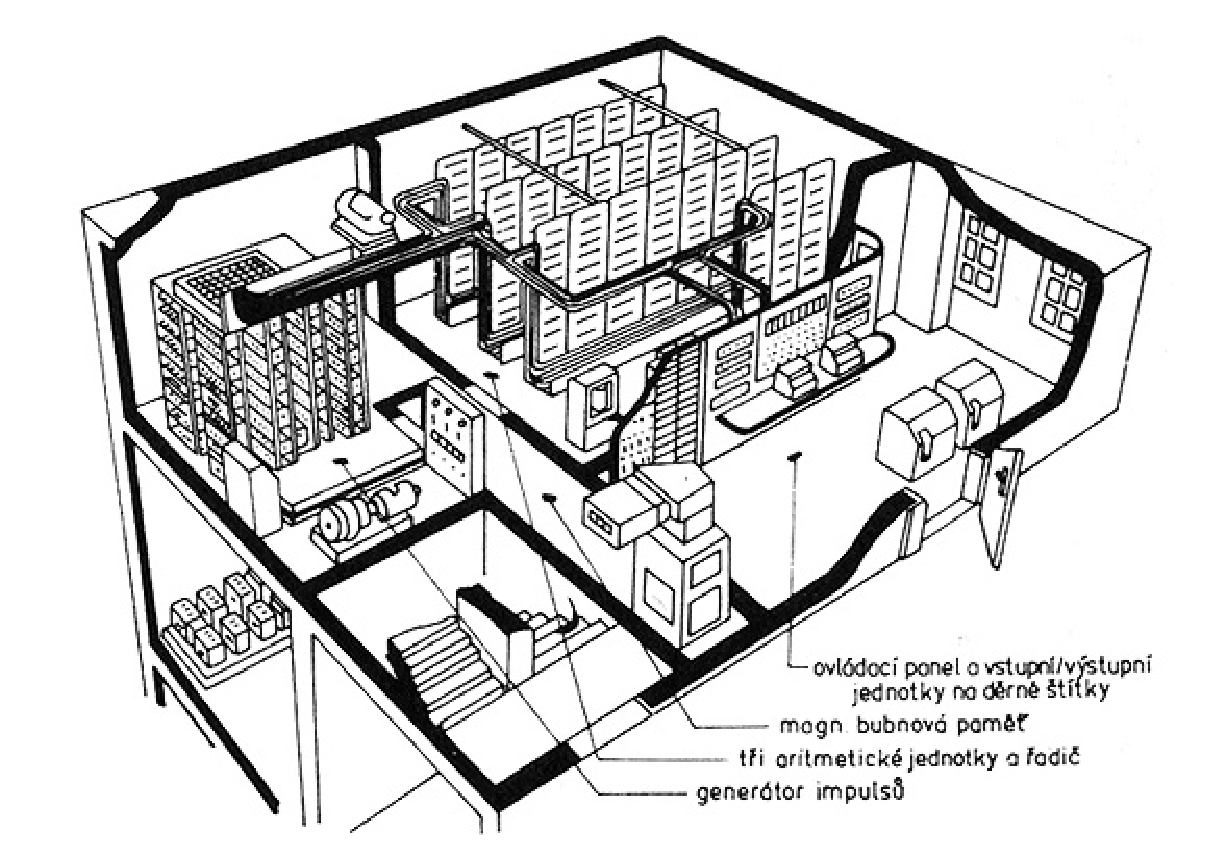
\includegraphics{schema-pocitace-sapo.eps}}
        \end{center}
    \end{frame}
\subsection{Specifika a rarity}
    \begin{frame}
        \frametitle{Specifika a rarity}
        \begin{itemize}
            \item První chybám odolný počítač na světě
            \item Místo elektronek použita relé
            \begin{itemize}
                \item Z důvodů výrobních kapacit ČSSR (použito 7 tisíc relé)
                    \begin{itemize}
                        \item Elektronky jsme v té době vyrobit neuměli
                    \end{itemize}
                \item Nespolehlivost relé je bohužel značná
            \end{itemize}
            \item Výkon 10 tisíc operací za hodinu (3 za vteřinu), ale!
            \begin{itemize}
                \item S 32bitovou přesností
                \item Možností výpočtů v plovoucí desetinné čárce
            \end{itemize}
        \end{itemize}
    \end{frame}
\subsection{Nové technologie}
    \begin{frame}
        \frametitle{Nové technologie}
        \begin{itemize}
            \item Tři aritmeticko-logické jednotky
                \begin{itemize}
                    \item Kvůli nespolehlivým relé
                    \item Z tohoto důvodu odolnost vůči chybám
                \end{itemize}
            \item Duplicitní zápis dat
                \begin{itemize}
                    \item Z důvodů Nespolehlivosti zápisových zařízení
                \end{itemize}
        \end{itemize}
    \end{frame}
\section{Závěr}
\subsection{Zdroje}
    \begin{frame}
        \frametitle{Děkuji za pozornost}
        \begin{itemize}
            \item Požité zdroje (informace a obrázek)
                \begin{itemize}
                    \item \textit{Antonín Svoboda\,--\,průkopník čš. výpočetní techniky} [online]. Mrg. Petr Kovář (Česká Republika): Historie výpočetní techniky v Československu. [cit. 2015-5-5]. Dostupné z http://www.historiepocitacu.cz/prukopnik-pocitacu-antonin-svoboda.html
                    \item \textit{Příchod hackerů: příběh profesora Svobody potřetí} [online]. Lukáš Erben (Česká Republika): Root.cz. [cit. 2015-5-5]. Dostupné z http://www.root.cz/clanky/prichod-hackeru-pribeh-profesora-svobody-potreti
                \end{itemize}
        \end{itemize}
    \end{frame}
\end{document}
